\documentclass[10pt]{article}
\usepackage{graphicx}
\usepackage{float}
\usepackage{array}
\addtolength{\oddsidemargin}{-.875in}
	\addtolength{\evensidemargin}{-.875in}
	\addtolength{\textwidth}{1.75in}

	\addtolength{\topmargin}{-.875in}
	\addtolength{\textheight}{1.75in}
\renewcommand{\baselinestretch}{0.97}
\title{Assignment 1}
\author {Ansh Prakash, 2016CS10367}

\date{Due date: January 13, 2020, 11:55pm IST}

\begin{document}

\maketitle

\section{Answer 1}
\subsection{ER Diagram}
%%% Fill in your content here.
\begin{figure}[h]
  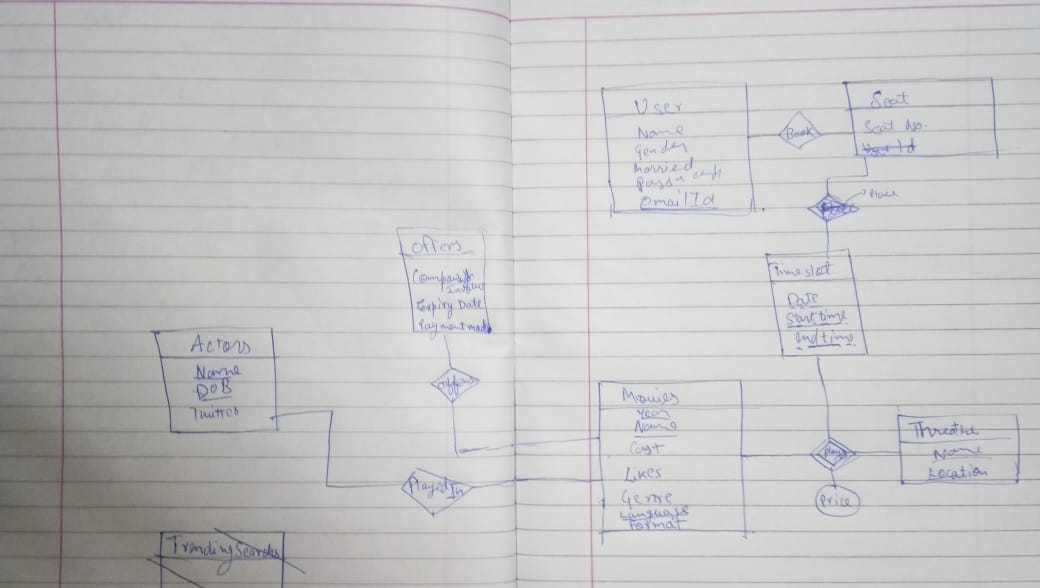
\includegraphics[width=10cm]{ER.jpeg}
  \caption{ER Diagram.}
  \label{fig:boat1}
\end{figure}


\subsection{Set of relations}
%%% Fill in your content here.

\begin{center}
 \begin{tabular}{| m{6em} | m{8cm}|} 
 \hline
 Entity & Attributes \\ [1ex] 
 \hline
 Movies & Year, Name, Cast, Likes, Genre, Language, Format \\
 Threatre & Name, Location \\
 TimeSlot & Date, Start\_time, End\_time \\
 Seat & SeatNo \\
 User & Name, Gender, Married, Password, emailId \\
 Offers & CompanyInvolved, ExpiryDate,PaymentMode \\
 Actor & Name, DoB, TwitterAccount \\

 PlayedIn & Year, Name, Cast, Likes, Genre, Language, Format, ActorName, DoB, Twitter \\
 Plays & Name, Location, Year, Name, Cast, Likes, Genre, Language, Format, Date, Start\_time, End\_time  \\
 Place & Date, Start\_time, End\_time, SeatNo \\
 Book & SeatNo, Name, Gender, Married, Password, emailId \\
 offers & CompanyInvolved, ExpiryDate,PaymentMode, Year, Name, Cast, Likes, Genre, Language, Format \\
 
 \hline
 
\end{tabular}
\end{center}


\subsection{Keys and FDs}
%%% Fill in your content here.
\begin{center}
 \begin{tabular}{| m{6em} | m{8cm}| m{8cm}|} 
 \hline
 Entity & Keys & FD\\ [1ex] 
 \hline
 Movies & Year, Name &  Cast, Likes, Genre, Language, Format \\
 Threatre & Name, Location & -\\
 TimeSlot & Date, Start\_time, End\_time & - \\
 Seat & SeatNo & - \\
 User & emailId & Name, Gender, Married, Password \\
 Offers & CompanyInvolved, ExpiryDate,PaymentMode & - \\
 Actor & Name, DoB & TwitterAccount\\
 \hline 
 \end{tabular}
\end{center}



\subsection{Sample Data}
%%% Fill in your content here.

\subsection{List of various relationships}
%%% Fill in your content here.

\begin{center}
 \begin{tabular}{| m{6em} | m{8cm}|} 
 \hline
 RelationShip & Entity \\ [1ex] 
 \hline
 Weak entity set & TimeSlot, Seat \\
 Non-binary relationship & Plays \\
 Hierarchical relationships & - \\
 referential constraints & Threatre, User \\ 
 
 \hline
 
\end{tabular}
\end{center}


\section{Answer 2}
%%% Fill in your content here.

\begin{center}
 \begin{tabular}{| m{6em}|} 
 \hline
 Universal Table \\ [1ex] 
 \hline
 Year, MovieName, Cast, Likes, Genre, Language, Format , ActorName, DoB,Twitter, ThreatreName, Location \\
 
 \hline
 
\end{tabular}
\end{center}

2NF ,3NF,BCNF all three at the same time


\begin{tabular}{| m{6em} | m{8cm}|} 
 \hline
 Table1 \\ [1ex] 
 \hline
 Year, Name, Cast, Likes, Genre, Language, Format, TreatreName, Location \\ 
 \hline
 
\end{tabular}


\begin{tabular}{| m{6em} | m{8cm}|} 
 \hline
 Table2 \\ [1ex] 
 \hline
 Year, Name, Cast, Likes, Genre, Language, Format, ActorName, DoB, TwitterAccount \\ 
 \hline 
 
\end{tabular}


\begin{tabular}{| m{6em} | m{8cm}|} 
 \hline
 Table3 \\ [1ex] 
 \hline
 Year, Name, Cast, Likes, Genre, Language, Format \\ 
 \hline 
 
\end{tabular}


\begin{tabular}{| m{6em} | m{8cm}|} 
 \hline
 Table4 \\ [1ex] 
 \hline
  ActorName, DoB, TwitterAccount \\ 
 \hline 
 
\end{tabular}


 \begin{tabular}{| m{6em} | m{8cm}|} 
 \hline
 Table5 \\ [1ex] 
 \hline
  THreatreName, Location \\ 
 \hline 
 
\end{tabular}






\section{Answer 3}
\subsection{Schema}
id	rated	created\_at	last\_move\_at	turns	victory\_status	winner\\	increment\_code	white\_id	white\_rating	black\_id	black\_rating	moves\\	opening\_eco	opening\_name	opening\_ply

%%% Fill in your content here.
\subsection{Various insert modes}
%%% Fill in your content here.
\subsubsection{Bulk Load}
%%% Fill in your content here.

sudo -u postgres psql
create database dbhw1;
\c dbhw1;
 create table hw1\_table (c1 varchar,c2 varchar,c3 varchar,c4 varchar,c5 varchar,c6 varchar,c7 varchar,c8 varchar,c9 varchar,c10 varchar,c11 varchar,c12 varchar,c13 varchar,c14 varchar,c15 varchar,c16 varchar);
COPY hw1\_table FROM '/home/ansh/8thSem/COL362/homework/games.csv' WITH (FORMAT csv);


\subsubsection{Insert statements}
%%% Fill in your content here.

\subsubsection{using JDBC}
%%% Fill in your content here.
\subsection{Statistics}
%%% Fill in your content here.
Dataset: games.csv 


\section{Answer 4}
%%% Fill in your content here.

\end{document}

